\documentclass[tikz,border=6pt]{standalone}
\usepackage{fontspec}
\setsansfont{Arial}
\begin{document}
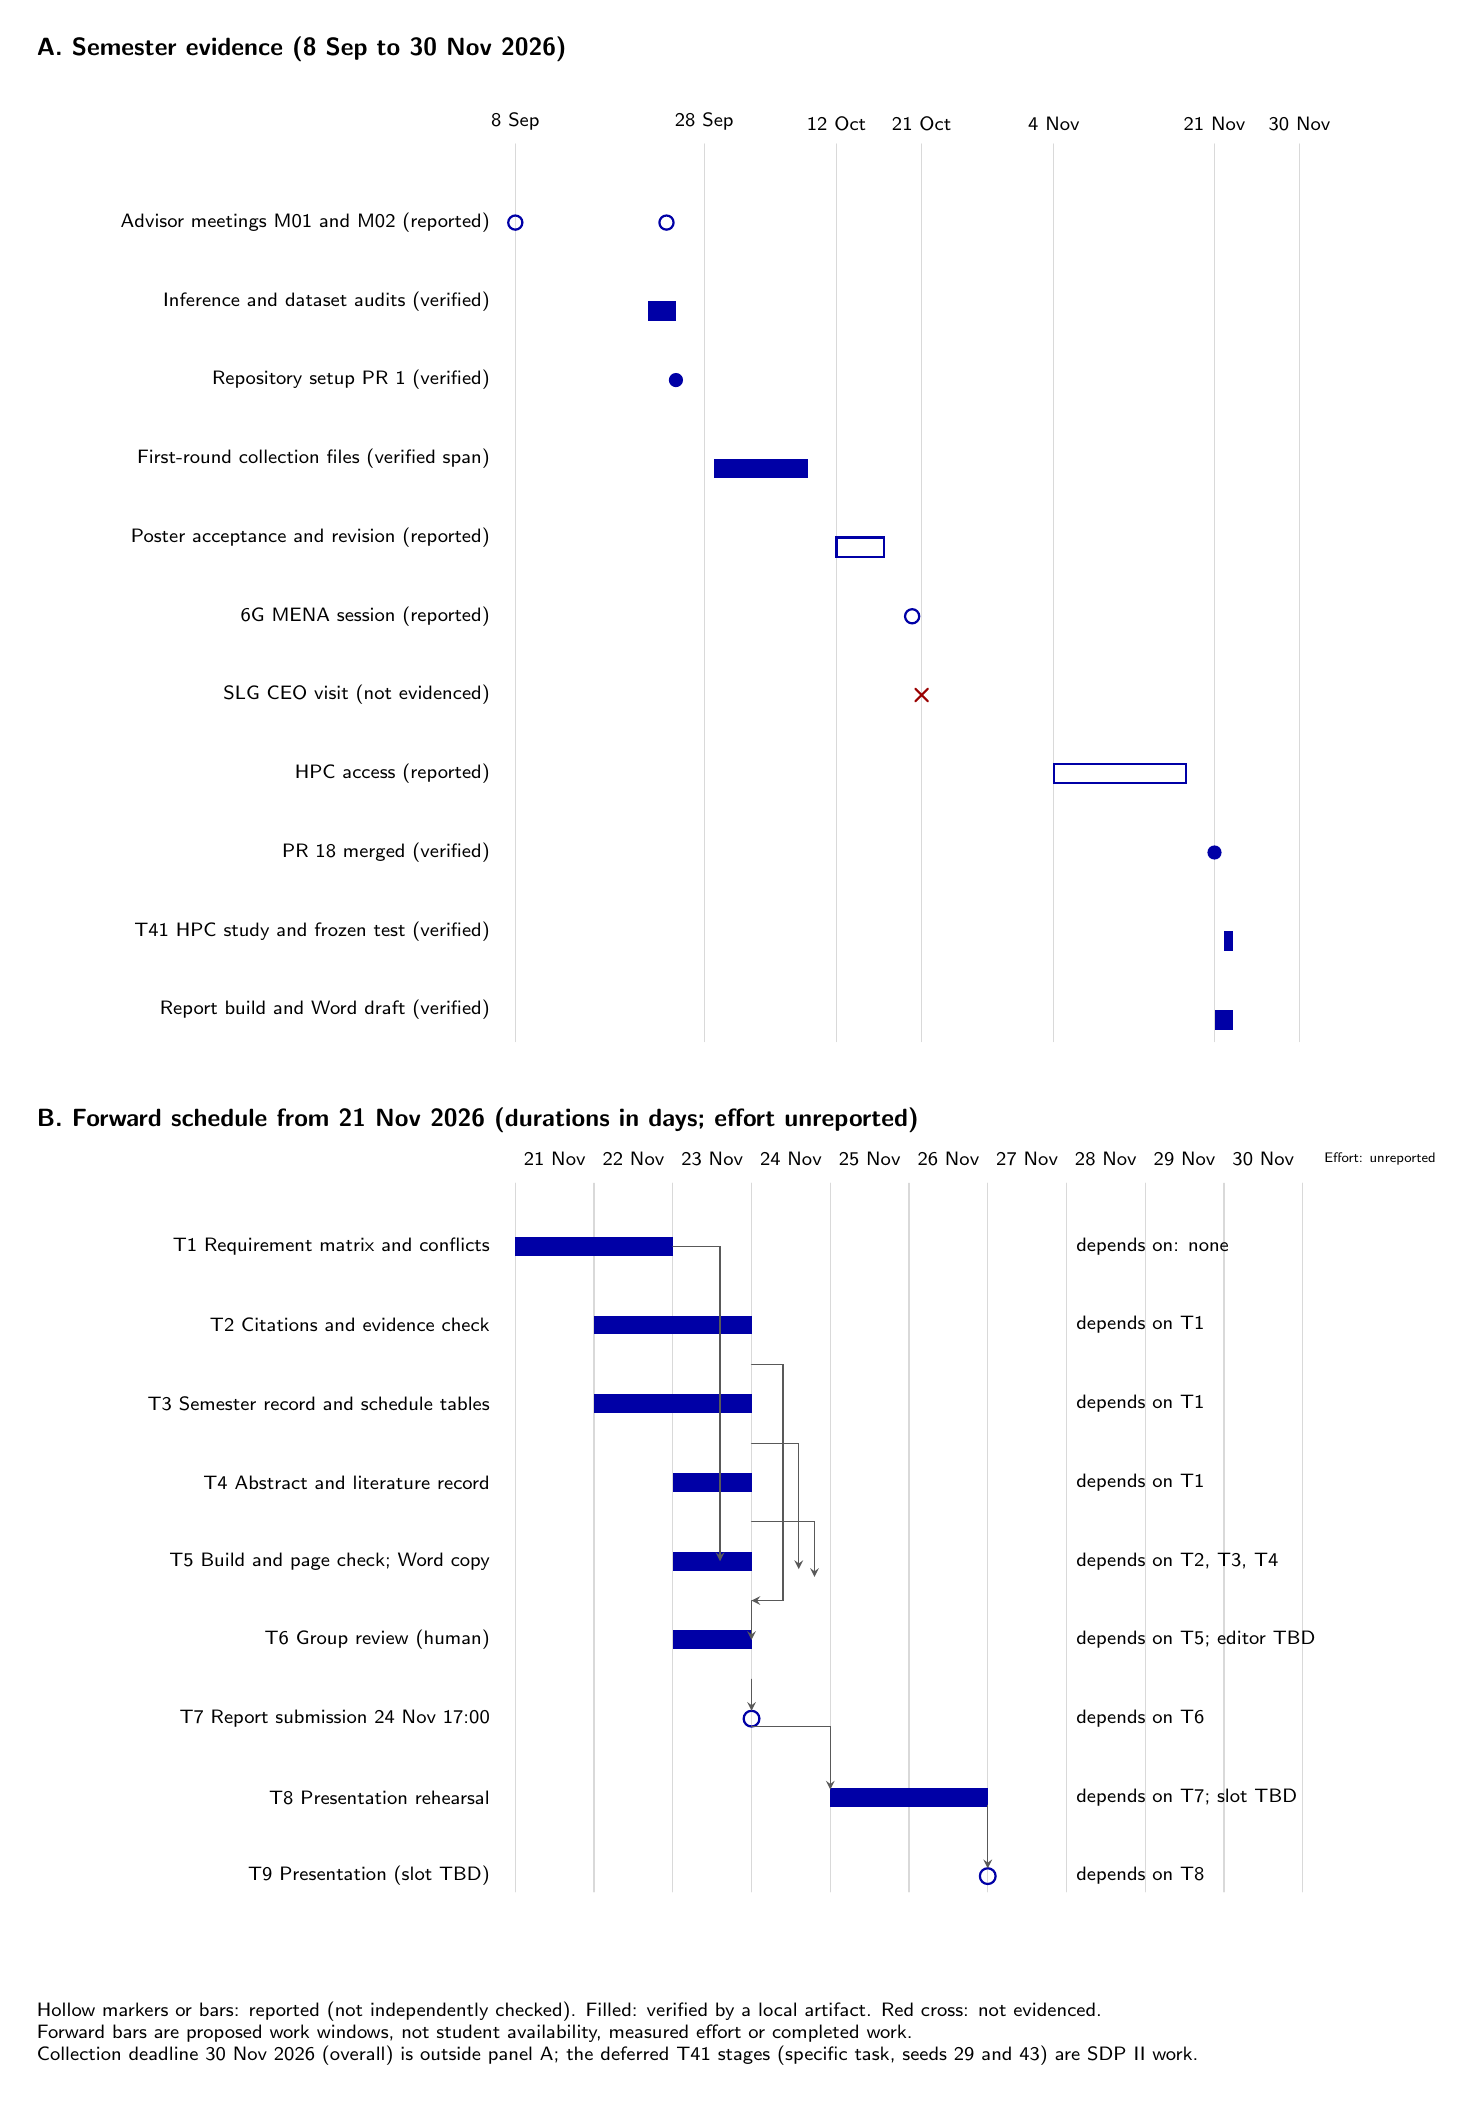
\begin{tikzpicture}[font=\sffamily\scriptsize, >=stealth, line cap=round]
% Panel A: semester evidence. Day 0 = 8 Sep 2026; 0.12 cm per day.
% Markers are dates of recorded events, not effort or hours.
\def\sA{0.12}
\node[anchor=west,font=\sffamily\small\bfseries] at (-6.2,1.2){A. Semester evidence (8 Sep to 30 Nov 2026)};
\foreach \d/\lab in {0/8 Sep,20/28 Sep,34/12 Oct,43/21 Oct,57/4 Nov,74/21 Nov,83/30 Nov}{
  \draw[gray!30] (\sA*\d,0)--(\sA*\d,-11.4);
  \node[anchor=south,rotate=0] at (\sA*\d,0.05){\lab};}
\foreach \y/\lab in {-1/Advisor meetings M01 and M02 (reported),-2/Inference and dataset audits (verified),-3/Repository setup PR 1 (verified),-4/First-round collection files (verified span),-5/Poster acceptance and revision (reported),-6/6G MENA session (reported),-7/SLG CEO visit (not evidenced),-8/HPC access (reported),-9/PR 18 merged (verified),-10/T41 HPC study and frozen test (verified),-11/Report build and Word draft (verified)}{
  \node[anchor=east] at (-0.2,\y){\lab};}
% Milestones: filled = verified, hollow = reported, cross = not evidenced
\foreach \d in {0,16}{\draw[blue!65!black,thick] (\sA*\d,-1) circle[x radius=0.09,y radius=0.09];}
\fill[blue!65!black] (\sA*14,-2) rectangle (\sA*17,-2.25);
\fill[blue!65!black] (\sA*17,-3) circle[x radius=0.09,y radius=0.09];
\fill[blue!65!black] (\sA*21,-4) rectangle (\sA*31,-4.25);
\draw[blue!65!black,thick] (\sA*34,-5) rectangle (\sA*39,-5.25);
\draw[blue!65!black,thick] (\sA*42,-6) circle[x radius=0.09,y radius=0.09];
\draw[red!60!black,thick] (\sA*43-0.08,-7.08)--(\sA*43+0.08,-6.92);
\draw[red!60!black,thick] (\sA*43-0.08,-6.92)--(\sA*43+0.08,-7.08);
\draw[blue!65!black,thick] (\sA*57,-8.12) rectangle (\sA*71,-7.88);
\fill[blue!65!black] (\sA*74,-9) circle[x radius=0.09,y radius=0.09];
\fill[blue!65!black] (\sA*75,-10) rectangle (\sA*76,-10.25);
\fill[blue!65!black] (\sA*74,-11) rectangle (\sA*76,-11.25);
% Panel B: forward schedule from 21 Nov 2026. Day 0 = 21 Nov; 1.0 cm per day.
\node[anchor=west,font=\sffamily\small\bfseries] at (-6.2,-12.4){B. Forward schedule from 21 Nov 2026 (durations in days; effort unreported)};
\foreach \d in {0,...,9}{
  \pgfmathtruncatemacro{\day}{21+\d}
  \draw[gray!30] (\d,-13.2)--(\d,-22.2);
  \node[anchor=south] at (\d+0.5,-13.1){\day\ Nov};}
\draw[gray!30] (10,-13.2)--(10,-22.2);
\node[anchor=south west,font=\sffamily\tiny] at (10.15,-13.1){Effort: unreported};
% Task rows: name, start, end (days), dependency text
\foreach \y/\lab in {-14/T1 Requirement matrix and conflicts,-15/T2 Citations and evidence check,-16/T3 Semester record and schedule tables,-17/T4 Abstract and literature record,-18/T5 Build and page check; Word copy,-19/T6 Group review (human),-20/T7 Report submission 24 Nov 17:00,-21/T8 Presentation rehearsal,-22/T9 Presentation (slot TBD)}{
  \node[anchor=east] at (-0.2,\y){\lab};}
\fill[blue!65!black] (0,-14.12) rectangle (2,-13.88);
\fill[blue!65!black] (1,-15.12) rectangle (3,-14.88);
\fill[blue!65!black] (1,-16.12) rectangle (3,-15.88);
\fill[blue!65!black] (2,-17.12) rectangle (3,-16.88);
\fill[blue!65!black] (2,-18.12) rectangle (3,-17.88);
\fill[blue!65!black] (2,-19.12) rectangle (3,-18.88);
\draw[blue!65!black,thick] (3,-20) circle[x radius=0.1,y radius=0.1];
\fill[blue!65!black] (4,-21.12) rectangle (6,-20.88);
\draw[blue!65!black,thick] (6,-22) circle[x radius=0.1,y radius=0.1];
% Dependencies
\draw[->,gray!70!black] (2,-14)--(2.6,-14)--(2.6,-18);
\draw[->,gray!70!black] (3,-15.5)--(3.4,-15.5)--(3.4,-18.5)--(3,-18.5);
\draw[->,gray!70!black] (3,-16.5)--(3.6,-16.5)--(3.6,-18.1);
\draw[->,gray!70!black] (3,-17.5)--(3.8,-17.5)--(3.8,-18.2);
\draw[->,gray!70!black] (3,-18.5)--(3,-19.0);
\draw[->,gray!70!black] (3,-19.5)--(3,-19.9);
\draw[->,gray!70!black] (3,-20.1)--(4,-20.1)--(4,-20.9);
\draw[->,gray!70!black] (6,-21.1)--(6,-21.9);
% Responsibility and dependency notes
\node[anchor=west] at (7.0,-14){depends on: none};
\node[anchor=west] at (7.0,-15){depends on T1};
\node[anchor=west] at (7.0,-16){depends on T1};
\node[anchor=west] at (7.0,-17){depends on T1};
\node[anchor=west] at (7.0,-18){depends on T2, T3, T4};
\node[anchor=west] at (7.0,-19){depends on T5; editor TBD};
\node[anchor=west] at (7.0,-20){depends on T6};
\node[anchor=west] at (7.0,-21){depends on T7; slot TBD};
\node[anchor=west] at (7.0,-22){depends on T8};
\node[anchor=west,align=left] at (-6.2,-24){Hollow markers or bars: reported (not independently checked). Filled: verified by a local artifact. Red cross: not evidenced.\\Forward bars are proposed work windows, not student availability, measured effort or completed work.\\Collection deadline 30 Nov 2026 (overall) is outside panel A; the deferred T41 stages (specific task, seeds 29 and 43) are SDP II work.};
\end{tikzpicture}
\end{document}
